\documentclass [11pt]{article}

\usepackage[italian]{babel}
\usepackage[utf8]{inputenc}

\usepackage{graphicx}

\begin{document}
\title{Web Architectures: Project report}
\date{2010/2011}
\author{Enrico Sartori (138531)}
\maketitle
\tableofcontents


\section{Introduction}
The project proposed is an implementation of a small hotel administration
suite. The main usage purpose of this software is to help the hotel staff
in managing arrivals, checkouts and reservations.

The main technologies used for developing this project are the ones
provided by the J2EE framework. In fact the server side of the application
is implemented using EJB 3.0, the storage and persistence layer is managed
by the Hibernate framework using MySql as a database.

For the Client side, the GWT toolkit has been used, in order to keep an
unity of language (Java) across the various component of this project and
to experiment with this toolkit.
The usage of GWT as a choice for implementing the client determines the
large use of AJAX technology.

\section {Use cases}
The system is intended to operate inside an organization, in order to
give to different users from different locations, the possibility to
perform the hotel administration tasks.

The application is thought to be similar to a common desktop application,
but, running inside a browser, overcomes portability and compatibility
issues.

There are two main phases characterizing the usage of the system,
configuration and reception tasks.

The main use cases for the configuration phase are:
\begin{itemize}
\item Create the prices for different periods and treatments (Full board,
half board and Bed and breakfast)
\item Create the list of items which a customer can purchase while
spending his holidays
\item Updating the user list
\item Define variations on the pricelist, like discounts or extra charge
(defined in percentage ora absolute value)
\end{itemize}

The reception tasks are summarized by the following list:
\begin{itemize}
\item Store arrival of customers
\item Perform checkout of departing customers
\item Manage reservations
\item Store items acquire by customers
\end{itemize}

The above tasks are summarized by Fig. \ref{fig:uses}.

\begin {figure}[h]
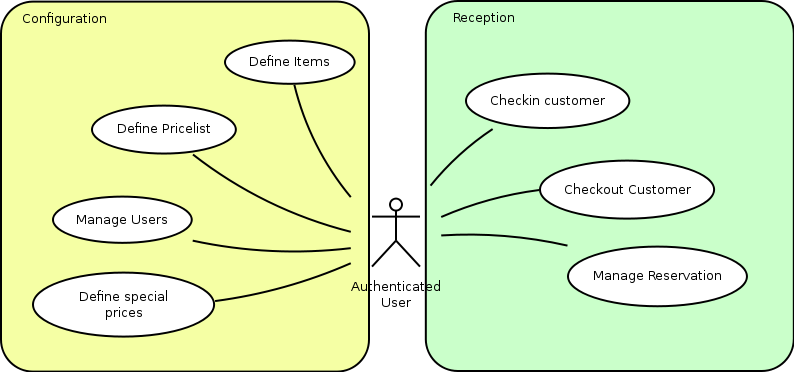
\includegraphics[width=\textwidth]{images/uses.png}
\caption {Use cases for the HotelBoss software}
\label{fig:uses}
\end {figure}

\section{Patterns used}
One of the main focus of the project is to experiment with the
implementation of different programming patterns, integrating them into a
functional architecture.
Therefore a particular attention has been devoted to the realization of
such patterns.

The following is a list of the most important pattern used developing the
project:
\begin{itemize}
\item DTO (Data Transfer Object)
\item DAO (Data Access Object)
\item Session Facade
\item Model View Controller
\item Business delegate
\end{itemize}

\subsection{Data Transfer Object}
This pattern covers the exchange of objects between the client and the
server, an between the various EJBs inside the server.
It's implemented through the encapsulation of the data inside a
Serializable object, easily transmissible through a network.

\subsection{Data Access Object}
The storage and management of the data in the database, and therefore the
communication with the Hibernate layer is brought by a set of EJBs,
visible only on the server side, which expose the operations to be
performed on the data.

In this way is possible to maintain a clear separation between the
business logic and the data layer, in fact all the operation on the data
layer are performed by the DAOs transparently to the server
implementation.

\subsection{Session facade}
In order to limit the overhead of calling many different EJBs from the
client, this pattern suggest to implement just one frontier Bean, exposing
the methods needed by the client.

The implementation given in this project is based on the realization of
two frontier Beans: one for the configuration phase and the other for the
Reception one.

\subsection {Model View Controller}
All the client views in the project are implemented following the MVC
pattern. Each one is composed by three classes, a View, a Model and a
Controller.

As the pattern states the only model interacts with the data, while the
view just gives a representation of it.
The controller class is called to react to the user inputs, updating the
view and the models state.

\subsection{Business Delegate}
In order to ease the communication between the client and the server this
pattern suggest to implement a class which performs all the calls,
centralizing acting as a proxy to the server.

In this project each view, treated as an independent module, has its own
Business Delegate, implemented by the model tier of the module. This class
performs all the calls to the services exposed by the server tier.

\section{Architecture}
This section describes the architecture of the system, illustrating the
development choices taken. A high level picture of the project is depicted
in image \ref{fig:arch}

\begin{figure}[h]
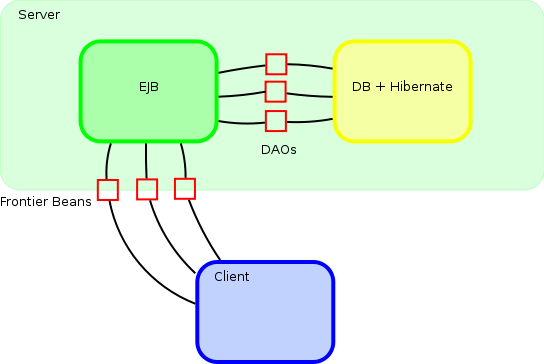
\includegraphics[width=\textwidth]{images/arch.png}
\caption {High level view of the Architecture}
\label {fig:arch}
\end{figure}

\subsection{Business Logic}
The business logic tier of the project expose two stateless EJBs and one
stateful EJB. The stateless EJBs (classes Configuration and Reception) cover the configuration and reception
phase of the software usage, giving to the user the tools to update the
state of the suite.

The stateful bean (class Checkout), instead is used to perform the billing tasks.
A local stateless bean is also dedicated to perform computation of the prices
and the totals of a bill, being a series of operation which require some
effort.

A picture of the system architecture is represented in image
\ref{fig:class}

\subsection{Web Client}
The client is implemented using the GWT toolkit, therefore it makes large
use of the AJAX technology.

The webclient is organized as a series of modules, each one performs a
specific task. The implementation of these modules follows a common
pattern, in fact each one is implemented by three classes, realizing the
MVC pattern.

The communication with the server is performed through three classes
(HBConfiguration, HBReception and HBCheckout) which reflect the frontier
bean of the server.

\subsection{Persistence Layer}
The persistence layer is implemented through a series of local EJBs which
implement the DAO pattern.
In particular the dao package in the project contains all the classes and
the interfaces which compose these EJBs.

The database schema is depicted in Fig. \ref{fig:er}

\begin{figure}[h]
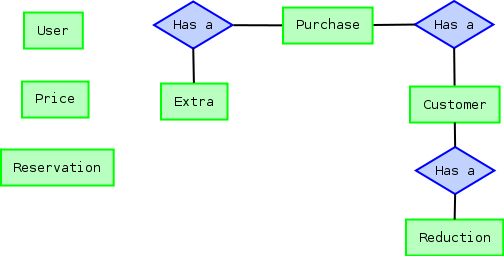
\includegraphics[width=\textwidth]{images/er.png}
\caption {ER diagram of the DB}
\label {fig:er}
\end{figure}


\begin{figure}[h]
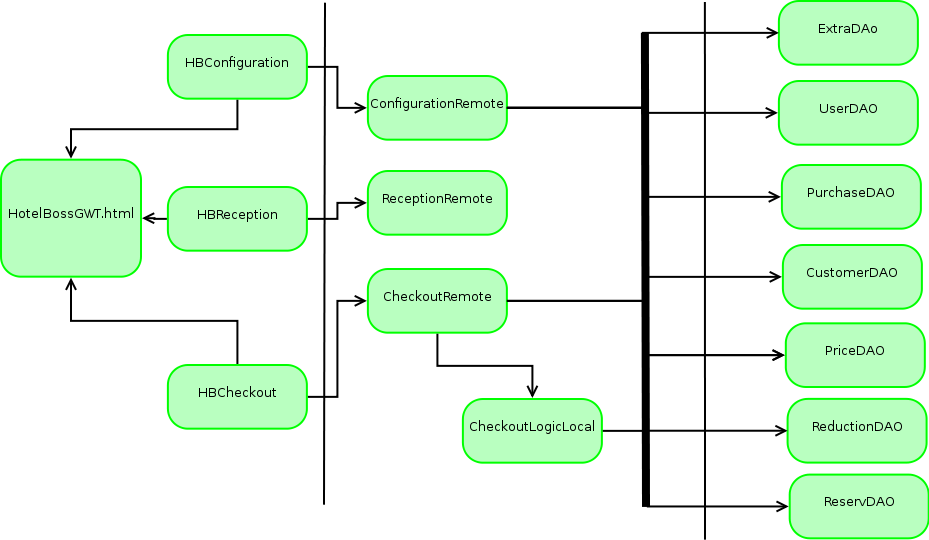
\includegraphics[width=\textwidth]{images/class.png}
\caption{Class diagram}
\label {fig:class}
\end{figure}


\section{Transactions}
The approach followed in defining the transaction policy, is to give great
importance to the operations regarding the billing process, while the
configuration part is considered a lower priority task.

In fact the configuration is basically a series of CRUD operation on the
database, storing the information needed for performing the Reception phase tasks.

\section{Security}
For securing the application the system relies on the JAAS framework, both
for the client and the server.

A different approach could have consisted in implementing a Stateful Bean which stores
the information of the user, permitting both to the client and the server
to check his authentication.

The main reason of this choice was to experiment with the JAAS system
offered by JBOSS.

\end{document}

